\documentclass[11pt]{article}
\usepackage[margin=1in]{geometry}
\usepackage{amsmath,amssymb,amsthm,mathtools,bm}
\usepackage{microtype}
\usepackage{booktabs}
\usepackage{graphicx}
\usepackage[hidelinks]{hyperref}
\usepackage{cleveref}
\usepackage[round]{natbib}
\bibliographystyle{plainnat}

\newtheorem{theorem}{Theorem}
\newtheorem{assumption}{Assumption}
\newtheorem{remark}{Remark}

\title{Reflexivity in Options Markets: \\
A Stochastic-Volatility Model with Dealer-Gamma Feedback, \\
Hopf Bifurcation Calculus, and a Pre-Registered Evaluation Framework}

\author{Mahimn Patel\\Independent Researcher\\\texttt{mahimn.patel.k@gmail.com}}

\date{April 2026}

\begin{document}
\maketitle

\begin{abstract}
We study a continuous-time Heston-like stochastic-volatility model in which the underlying spot price is coupled to its own option market through a dealer-gamma feedback channel, derived from the open-interest grid via a G\^arleanu--Pedersen--Poteshman \citep{garleanu2009demand} demand-pressure mapping. The model state is three-dimensional---spot $S_t$, instantaneous variance $v_t$, and a low-pass-filtered log-spot memory variable $z_t$---and reduces to standard time-dependent Heston \citep{heston1993} at zero coupling. Our contribution is the synthesis of three previously separate ingredients into a single analytical and computational object: (i) a continuous-time SV backbone with explicit dealer-gamma drift, (ii) a formal Hopf bifurcation calculus on the deterministic skeleton with first Lyapunov coefficient $\ell_1$ and Khasminskii-style stochastic shift $\Lambda$, and (iii) a pre-registered evaluation protocol for RL-trained hedging agents trained inside the simulator. For a representative dimensionless calibration we obtain a critical coupling $\kappa^\star \approx 0.8964$, angular frequency $\omega^\star \approx 0.5724$~rad/yr, and first Lyapunov coefficient $\ell_1 \approx -0.025 < 0$, so the bifurcation is supercritical: an attracting limit cycle in volatility is born for $\kappa > \kappa^\star$. The 2D reduction (without $z_t$) has an upper-triangular Jacobian and admits only a saddle-node onset, recovering the discrete-time recursion of \citet{dai2025gamma}; the 3D extension is what unlocks the Hopf. The closest model-structure precedent \citep{halperin2025marketron} does not perform the bifurcation analysis we provide. For the natural parametric specification with log-normal open-interest in moneyness, we obtain a closed-form Hopf threshold and a closed-form $\ell_1$, exposing a parametric phase boundary in $(\sigma_q, \gamma)$ space.
\end{abstract}

\section{Introduction}
\label{sec:intro}

Real options markets exhibit endogenous volatility cycles that pure stochastic-volatility (SV) models cannot reproduce. The empirical anchor is \citet{hardiman2013}, who fit Hawkes-process branching ratios to E-mini mid-price changes over 1998--2011 and find $n \approx 1$ throughout---the precise critical edge between sub- and super-criticality of endogenous events. \citet{soros2009reflexivity} and \citet{bouchaud2011endo} are the conceptual antecedents; \citet{filimonov2012} formalised the reflexivity-quantification programme that \citet{hardiman2013} executed. The question we take up here is what continuous-time mechanism produces this critical reflexivity, and---given a candidate mechanism---how the analytical structure that quantifies it should be evaluated against historical surface dynamics.

We contribute the following.
\begin{itemize}
\item A 3D reflexive SV simulator $(S_t, v_t, z_t)$ with explicit dealer-gamma feedback derived from the option open-interest grid via the \citet{garleanu2009demand} demand-pressure mapping. The variance backbone is Heston \citep{heston1993}; the memory equation $\dot z = -\alpha z + \beta \log(S/S_0)$ closes the leverage feedback channel that the 2D reduction lacks.
\item A Hopf bifurcation theorem (Theorem~\ref{thm:hopf}) for the deterministic skeleton at $\kappa^\star$ given by Liu's criterion (Routh--Hurwitz with one zero), with closed-form first Lyapunov coefficient $\ell_1$ and closed-form Hopf threshold for log-normal open-interest in moneyness (Eqs.~\ref{eq:lognorm-kappastar}--\ref{eq:lognorm-ell1}).
\item A numerical phase diagram in $(\xi, \rho, \sigma_v)$ together with the Khasminskii-style stochastic-Hopf shift $\Lambda$ and a parametric phase boundary in $(\sigma_q, \gamma)$ space.
\item A pre-registration of the empirical evaluation pipeline (sliced-Wasserstein-2 over 21-day surface windows, $\kappa$-sensitivity slope, Hopf-frequency spectral test) at git commit \texttt{268c061} with an OpenTimestamps Bitcoin-anchored proof, in the spirit of \citet{camerer2018} adapted for computational finance.
\end{itemize}

\paragraph{Closest precedents.} \citet{halperin2025marketron} (Marketron) share the model-structural axis---continuous-time SDE, memory channel, options-aware---but do not perform the bifurcation analysis. \citet{dai2025gamma} share the dealer-gamma axis but produce a saddle-node onset (the 2D reduction's instability), not a Hopf. \citet{hesuttergonon2025} (NeurIPS 2025) share the RL-with-environmental-sweep idea but train separate agents per grid point rather than reporting the slope at an anchor. The continuous-time HAM-Hopf precedents \citep{heli2009,chiarellahehommes2006} use delay-differential heterogeneous-belief models without an options-grid feedback channel; the discrete-time \citet{brockhommeswagener2009} ``more hedging instruments may destabilize markets'' result is the methodological template for derivative-driven Neimark--Sacker (Hopf-for-maps) bifurcations. The hedger-flow-feedback foundations are \citet{freystremme1997,sircarpapanicolaou1998,platenschweizer1998}. \Cref{sec:hopf,sec:eval,sec:mechanism} make these contrasts precise.

\paragraph{Roadmap.} \Cref{sec:model} states the model. \Cref{sec:hopf} proves Theorem~\ref{thm:hopf} and gives the closed-form $\ell_1$ for log-normal OI. \Cref{sec:phase} reports the numerical phase diagram. \Cref{sec:eval} describes the pre-registered evaluation framework. \Cref{sec:mechanism} reports the mechanism decomposition against Marketron. \Cref{sec:conclusions} closes with the empirical-calibration roadmap. Code at \url{https://github.com/mahimn01/reflexive-options}; pre-registration anchored to commit \texttt{268c061}.

\section{The reflexive model}
\label{sec:model}

Let $S_t$ be the underlying spot price, $v_t$ the instantaneous variance, and $z_t$ a memory variable encoding low-pass-filtered price history. The reflexive system is
\begin{align}
\frac{dS_t}{S_t} &= \bigl(\mu + \kappa\, G(S_t, z_t, v_t)\bigr)\, dt + \sigma(S_t, v_t)\, dW^S_t, \label{eq:reflexive-S}\\
dv_t &= \bigl(\kappa_v(\theta_v - v_t) + \gamma\, z_t\bigr)\, dt + \xi \sqrt{v_t}\, dW^v_t, \label{eq:reflexive-v}\\
dz_t &= \bigl(-\alpha\, z_t + \beta\, \log(S_t / S_0)\bigr)\, dt, \label{eq:reflexive-z}\\
d\langle W^S, W^v\rangle_t &= \rho\, dt, \label{eq:reflexive-corr}
\end{align}
with $\kappa \geq 0$ the reflexive coupling, $\gamma \geq 0$ the leverage-feedback strength, $\alpha > 0$ the memory decay rate, $\beta$ dimensionless, and $G(\cdot)$ the aggregate dealer-gamma exposure derived from the option open-interest grid:
\begin{equation}
G(S, t) \;=\; \sum_{K, T} q_{K, T}\,\Gamma_{K, T}(S, t)\,\mathrm{sign}(K, T),
\label{eq:G-aggregator}
\end{equation}
where $q_{K, T}$ is open interest at strike $K$ and maturity $T$, $\Gamma_{K, T}$ is per-contract Black--Scholes gamma, and the sign convention follows the SqueezeMetrics dealer-net convention \citep{squeezemetrics2017}. When $\kappa = \gamma = 0$, the system collapses to standard Heston \citep{heston1993}; this collapse is verified numerically in \texttt{tests/test\_simulator.py}.

For numerical stability of the variance scheme we use the full-truncation Euler of \citet{lordkoekkoekvandijk2010}; the empirical reference for the dealer-gamma magnitudes in $G$ is \citet{barbonburaschi2021,dimerakervilkov2024} (calibration to SPX 0DTE / dealer-gamma data, which we will use at Phase~4 of the empirical pipeline).

\paragraph{Why three states.} A reduced 2D specification---dropping $z_t$ and the $\gamma z$ term---has Jacobian in deviation variables $(y, u)$ around an equilibrium of the form
\[
J_{2D}(\kappa) = \begin{pmatrix} a(\kappa) & b(\kappa) \\ 0 & -\kappa_v \end{pmatrix},
\]
which is upper triangular: eigenvalues $\{a(\kappa), -\kappa_v\}$ are always real, and only saddle-node / transcritical bifurcations are admissible as $a(\kappa)$ crosses zero. This recovers the static onset of \citet{dai2025gamma}. To Hopf, the feedback must flow in both directions: price $\to$ variance and variance $\to$ price. The minimal modification is the leverage channel $\gamma z$ together with the auxiliary memory equation \eqref{eq:reflexive-z}---structurally analogous to the memory variable in the Marketron quasi-particle SDE \citep{halperin2025marketron} though with very different mechanistic content.

\section{Hopf bifurcation theorem and closed-form \texorpdfstring{$\ell_1$}{ell-1}}
\label{sec:hopf}

\subsection{Equilibria and Jacobian}
\label{sec:hopf-jac}

Drop the Brownian terms and work in log-deviation variables $(y, u, z) = (\log(S/S^\star), v - \theta_v, z - z^\star)$ around the unique equilibrium $(S^\star, \theta_v, z^\star)$ defined by
\begin{equation}
\mu - \tfrac{1}{2}\sigma^2(S^\star, \theta_v) + \kappa\, G(S^\star, z^\star, \theta_v) = 0, \qquad z^\star = \frac{\beta}{\alpha}\log(S^\star/S_0). \label{eq:equilibrium}
\end{equation}
To linear order, the deterministic skeleton (\ref{eq:reflexive-S}--\ref{eq:reflexive-z}) becomes $\dot{\bm{x}} = J(\kappa)\, \bm{x}$ with $\bm{x} = (y, u, z)^\top$ and
\begin{equation}
J(\kappa) = \begin{pmatrix}
a(\kappa) & b(\kappa) & \kappa\, G_z \\
0 & -\kappa_v & \gamma \\
\beta & 0 & -\alpha
\end{pmatrix}, \label{eq:jacobian}
\end{equation}
where $a(\kappa) = \kappa\, G_x - \tfrac{1}{2}\partial_x\sigma^2$, $b(\kappa) = \kappa\, G_v - \tfrac{1}{2}\partial_v\sigma^2$, and $G_x, G_v, G_z$ denote partial derivatives of $G$ at the equilibrium.

\subsection{Routh--Hurwitz / Liu's criterion}
\label{sec:hopf-rh}

The characteristic polynomial of \eqref{eq:jacobian} is $P(\lambda; \kappa) = \lambda^3 + c_2(\kappa)\lambda^2 + c_1(\kappa)\lambda + c_0(\kappa)$, with
\[
c_2 = -a + \kappa_v + \alpha, \quad
c_1 = -a\kappa_v - a\alpha + \kappa_v\alpha - \kappa\, G_z\, \beta, \quad
c_0 = -a\kappa_v\alpha - \beta\bigl(\kappa\, G_z\, \kappa_v + b\,\gamma\bigr).
\]
A 3D system Hopfs iff (Liu's criterion, equivalent to Routh--Hurwitz with one zero):
\begin{equation}
c_2 > 0, \qquad c_0 > 0, \qquad c_1 c_2 - c_0 = 0, \qquad \frac{d}{d\kappa}\bigl[c_1 c_2 - c_0\bigr] \neq 0. \label{eq:hopf-condition}
\end{equation}
Define $H(\kappa) := c_1(\kappa)\, c_2(\kappa) - c_0(\kappa)$. The Hopf threshold is
\begin{equation}
\boxed{\;\kappa^\star = \{\kappa > 0 : H(\kappa) = 0,\; H'(\kappa) \neq 0,\; c_2(\kappa) > 0,\; c_0(\kappa) > 0\}.\;} \label{eq:kappa-star}
\end{equation}
At $\kappa = \kappa^\star$ the Jacobian has a pure imaginary eigenvalue pair $\lambda_\pm = \pm i\omega^\star$ with $\omega^\star = \sqrt{c_1(\kappa^\star)}$, plus a real eigenvalue $\lambda_3 = -c_2(\kappa^\star) < 0$.

\subsection{Theorem 1 and proof sketch}
\label{sec:hopf-thm}

\begin{theorem}[Hopf bifurcation in the gamma-coupled SV skeleton]
\label{thm:hopf}
Let the deterministic system (\ref{eq:reflexive-S}--\ref{eq:reflexive-z}) (with Brownian terms removed) satisfy:
\begin{description}
\item[(A1)] $G \in C^3$ and $\sigma^2 \in C^3$ in their arguments, with $\sigma^2$ bounded below by a positive constant.
\item[(A2)] There exists a locally unique equilibrium $(S^\star, \theta_v, z^\star)$ given by \eqref{eq:equilibrium} for every $\kappa$ in some interval $[0, \kappa_{\max}]$, in some open neighborhood of which the linearization \eqref{eq:jacobian} is non-degenerate. Multiple equilibria may exist globally; our analysis is local.
\item[(A3)] The map $\kappa \mapsto (a(\kappa), G_z, G_v)$ is $C^3$.
\item[(A4)] There exists $\kappa^\star \in (0, \kappa_{\max})$ satisfying \eqref{eq:kappa-star} with $\omega^\star := \sqrt{c_1(\kappa^\star)} > 0$.
\item[(A5)] The first Lyapunov coefficient $\ell_1(\kappa^\star) \neq 0$ \citep[eq.~3.20]{kuznetsov2004}.
\end{description}
Then the equilibrium undergoes a Hopf bifurcation at $\kappa = \kappa^\star$. Specifically:
\begin{enumerate}
\item For $\kappa$ in a one-sided neighbourhood of $\kappa^\star$ (sub- or super-critical depending on $\mathrm{sgn}\,\ell_1$), there exists a unique smooth family of periodic orbits $\Gamma_\kappa$ of period $T_\kappa = 2\pi/\omega^\star + O(\kappa - \kappa^\star)$ and amplitude proportional to $\sqrt{|\kappa - \kappa^\star|}$.
\item The orbits are stable iff $\ell_1(\kappa^\star) < 0$ (supercritical).
\item On $\Gamma_\kappa$, $u_t = v_t - \theta_v$ oscillates with amplitude proportional to $\sqrt{|\kappa - \kappa^\star|}$, providing endogenous volatility cycles.
\end{enumerate}
\end{theorem}

\begin{proof}[Proof sketch]
The eigenvalue pair $\lambda_\pm(\kappa)$ is smooth in $\kappa$ near $\kappa^\star$ by the implicit function theorem applied to $P(\lambda; \kappa) = 0$. Routh--Hurwitz gives $\mathrm{Re}\,\lambda_\pm(\kappa^\star) = 0$, and the transversality $H'(\kappa^\star) \neq 0$ translates to $\frac{d}{d\kappa}\mathrm{Re}\,\lambda_\pm \neq 0$. The centre manifold theorem \citep[Thm.~5.4]{kuznetsov2004} (see also \citealp{carr1981}) gives a smooth 2D invariant manifold tangent to the eigenspace of $\pm i\omega^\star$. Conjugating the restricted system to its Poincar\'e normal form and applying \citet[Thm.~3.3]{kuznetsov2004} yields claims (1)--(3).
\end{proof}

\subsection{Numerical anchor}
\label{sec:hopf-numerical}

The default \texttt{BifurcationConfig} in our experiments code does not exhibit a Hopf within the literature-prior $\kappa$ range when the dealer-gamma magnitudes are tuned to empirical scale---this is consistent with the empirical observation that real options markets sit \emph{near} but not \emph{across} $\kappa^\star$, in line with the $n \approx 1$ regime of \citet{hardiman2013}. For a worked numerical example we use a representative dimensionless regime with $\{G_x, G_v, G_z\} = \{0.5, -0.5, -0.5\}$, $\alpha = 0.5$/yr, $\beta = 1$, $\gamma = 0.5$, $\kappa_v = 2$/yr, and constant-volatility surrogate ($\partial_v\sigma^2 = 0$). The deterministic skeleton then satisfies:
\begin{table}[h]
\centering
\begin{tabular}{lr}
\toprule
Quantity & Value \\
\midrule
$\kappa^\star$ & $0.8964$ \\
$\omega^\star$ & $0.5724$ rad/yr \\
Third real eigenvalue $\lambda_3$ & $-2.052$ \\
First Lyapunov coefficient $\ell_1$ & $-2.53 \times 10^{-2}$ \\
\textbf{Bifurcation type} & \textbf{supercritical} ($\ell_1 < 0$) \\
\bottomrule
\end{tabular}
\caption{Canonical Hopf-exhibiting regime for the deterministic skeleton.}
\label{tab:hopf-canonical}
\end{table}

Supercriticality means an attracting limit cycle is born for $\kappa > \kappa^\star$ with amplitude proportional to $\sqrt{\kappa - \kappa^\star}$---i.e.\ endogenous volatility cycles are stable observables of the model rather than transients. The Khasminskii sphere-process estimator \citep{khasminskii1980,arnold1998,baxendale1994} for the stochastic-Hopf shift, evaluated by \texttt{experiments/lambda\_correction\_canonical} on the bare Heston-with-memory linearisation at the trivial $G \equiv 0$ equilibrium with the $\S\ref{sec:hopf-numerical}$ memory parameters, gives $|\Lambda(\kappa^\star)|$ on the order of $10^{-3}$ at both the canonical $(\xi, \rho) = (0.3, 0)$ and SPX-representative $(0.3, -0.7)$ configurations. The sign of $\Lambda$ depends sensitively on the open-interest configuration and on the specific equilibrium chosen; we therefore defer a definitive characterisation of the stochastic-Hopf shift to the empirical phase, and only use $|\Lambda| \cdot \varepsilon^2 \ll 1$ at calibration-noise scale to conclude that the deterministic threshold $\kappa^\star$ is the operationally relevant one. The shear-induced-correction prediction of \citet{engellambrasmussen2024} is consistent with this magnitude but is not validated in sign by the present finite-budget estimator.

\subsection{Closed-form \texorpdfstring{$\kappa^\star$}{kappa-star} and \texorpdfstring{$\ell_1$}{ell-1} for log-normal OI in moneyness}
\label{sec:hopf-closed-form}

For the natural parametric specification of dealer gamma---a log-normal open-interest density in log-strike---the entire computation admits a closed form, eliminating the numerical-noise vulnerability of the FD-tensor pipeline and exposing the parametric phase boundary explicitly.

Replace the discrete OI grid with the continuous density $q(\log K) = \frac{1}{\sigma_q\sqrt{2\pi}}\exp\bigl(-(\log K - \mu_q)^2/(2\sigma_q^2)\bigr)$. Take a single representative maturity $T_{\mathrm{eff}}$, sign convention $s \equiv +1$, and write $a := \log S$. The aggregator becomes
\begin{equation}
G(a, v) \;=\; \kappa_u \int_{-\infty}^{+\infty} q(\log K)\, \Gamma_{\mathrm{BS}}\!\left(S, K, T_{\mathrm{eff}}, \sqrt{v}\right)\, d(\log K). \label{eq:G-integral}
\end{equation}
Since Black--Scholes gamma at fixed $T = T_{\mathrm{eff}}$, $\sigma = \sqrt{v}$ is itself Gaussian in $\log K$, the standard Gaussian-product identity collapses \eqref{eq:G-integral} to
\begin{equation}
\boxed{\;G(a, v) \;=\; \mathcal{C}(v)\cdot e^{-a}\cdot \exp\!\biggl(-\frac{(a - m(v))^2}{2\,\tau^2(v)}\biggr),\;} \label{eq:G-closed-form}
\end{equation}
where
\begin{equation}
\mathcal{C}(v) = \frac{\kappa_u\, e^{-q_{\mathrm{div}} T_{\mathrm{eff}}}}{\sqrt{2\pi\,\tau^2(v)}}, \quad
\tau^2(v) = \sigma_q^2 + v\,T_{\mathrm{eff}}, \quad
m(v) = \mu_q - \bigl(r - q_{\mathrm{div}} + \tfrac{1}{2}v\bigr)\, T_{\mathrm{eff}}. \label{eq:G-coefficients}
\end{equation}
$G$ depends on $a$ and $v$ but not on $z$; the leverage channel $\gamma z$ in $\dot u$ keeps the $(2,3)$ Jacobian entry alive, so cross-coupling persists through the variance row even with $G_z = 0$.

With $G_z = 0$ and $\sigma^2 = v$ (so $\partial_y\sigma^2 = 0$, $\partial_v\sigma^2 = 1$), the Routh--Hurwitz polynomial $H(\kappa) = c_1 c_2 - c_0$ degree-collapses from cubic to quadratic in $\kappa$:\footnote{Throughout this closed-form section we write $G_y := \partial_a G$ for the partial of the dealer-gamma functional with respect to the deviation variable $y = a - a^\star$; this is identical to the $G_x$ of \cref{sec:hopf-jac} up to the choice of deviation symbol.}
\begin{equation}
H(\kappa) = G_y^2\,(\alpha + \kappa_v)\,\kappa^2 + \bigl(G_v\,\beta\gamma - G_y\,(\alpha + \kappa_v)^2\bigr)\,\kappa + \alpha\kappa_v(\alpha + \kappa_v) - \tfrac{1}{2}\beta\gamma. \label{eq:lognorm-H}
\end{equation}
Writing $A := \alpha + \kappa_v$, $M := \alpha\kappa_v$, $L := \beta\gamma$, the Hopf threshold is the smallest positive root of the quadratic:
\begin{equation}
\boxed{\;\kappa^\star \;=\; \frac{G_y\, A^2 - G_v\, L \;-\; \sqrt{(G_v L - G_y A^2)^2 - 4\,G_y^2 A\,(MA - L/2)}}{2\,G_y^2\,A}.\;} \label{eq:lognorm-kappastar}
\end{equation}
The discriminant in \eqref{eq:lognorm-kappastar} provides the first parametric phase boundary: when $D := (G_v L - G_y A^2)^2 - 4\,G_y^2 A\,(MA - L/2) < 0$, the system has no Hopf at any $\kappa$ and the deterministic skeleton is unconditionally stable.

The third-order partials of \eqref{eq:G-closed-form} at the equilibrium are explicit rational functions of $(\delta := a^\star - m(v^\star),\, \tau^2,\, T_{\mathrm{eff}})$, so the bilinear and trilinear tensors $B$, $C$ at $\kappa^\star$ admit a closed form. Substituting into the Kuznetsov formula
\begin{equation}
\ell_1(\kappa^\star) = \frac{1}{2\omega^\star}\,\mathrm{Re}\!\Bigl[\langle p, C(q, q, \bar q)\rangle - 2\langle p, B(q, J^{-1} B(q, \bar q))\rangle + \langle p, B(\bar q, (2i\omega^\star I - J)^{-1} B(q, q))\rangle\Bigr], \label{eq:lognorm-ell1}
\end{equation}
with $J q = i\omega^\star q$, $J^\top p = -i\omega^\star p$, $\langle p, q\rangle = 1$, yields a $\sim 30$-term rational in the $G$-partials $(G_y, G_v, G_{aa}, G_{av}, G_{vv}, G_{aaa}, G_{aav}, G_{avv}, G_{vvv})$ and $(\kappa_v, \alpha, \beta, \gamma)$. The implementation evaluates this in $\sim 50\,\mu$s per parameter tuple, with results matching the FD-tensor pipeline to better than $0.6\%$ relative on every parameter set tested.

At the canonical regime $(\sigma_q = 0.10, T_{\mathrm{eff}} = 0.25, \kappa_v = 2, \alpha = 0.05, \beta = 1, \gamma = 1, \mu_q = \log 100, v^\star = 0.04)$, \eqref{eq:lognorm-kappastar}--\eqref{eq:lognorm-ell1} give $\kappa^\star = 17.81$, $\omega^\star = 1.18$~rad/yr, $\ell_1 = -4.81 \times 10^{-1}$ (supercritical). The closed form is essentially noise-free; with it in hand, the sign of $\ell_1$ near the boundary contour is structurally certain rather than statistically inferred.

\section{Numerical phase diagram}
\label{sec:phase}

The full $(\kappa, \xi, \rho, \sigma_v)$ phase diagram is computed by sweeping $\kappa \in [0, 2]$ on a 401-point grid for each of $31 \times 21 \times 4 = 2{,}604$ cells over $(\xi, \rho, \sigma_v)$ at the \cref{sec:hopf-numerical} Hopf-exhibiting regime. The pair $(\xi, \rho)$ enters the deterministic Jacobian via the leading shear-induced correction $a_{\mathrm{eff}}(\kappa) = a(\kappa) + \tfrac{1}{2}\xi^2 \rho\, G_v$---an \citet{engellambrasmussen2024}-style projection of the small-noise stochastic Hopf onto the eigenvalue envelope. Wall-clock: $\sim 16$~s on a single M-series core. \Cref{fig:hopf-phase-diagram} renders the $(\xi, \rho)$ heatmap and four line cuts of $\kappa^\star(\sigma_v)$ at SPX-relevant $(\xi, \rho)$ probes.

\begin{figure}[t]
\centering
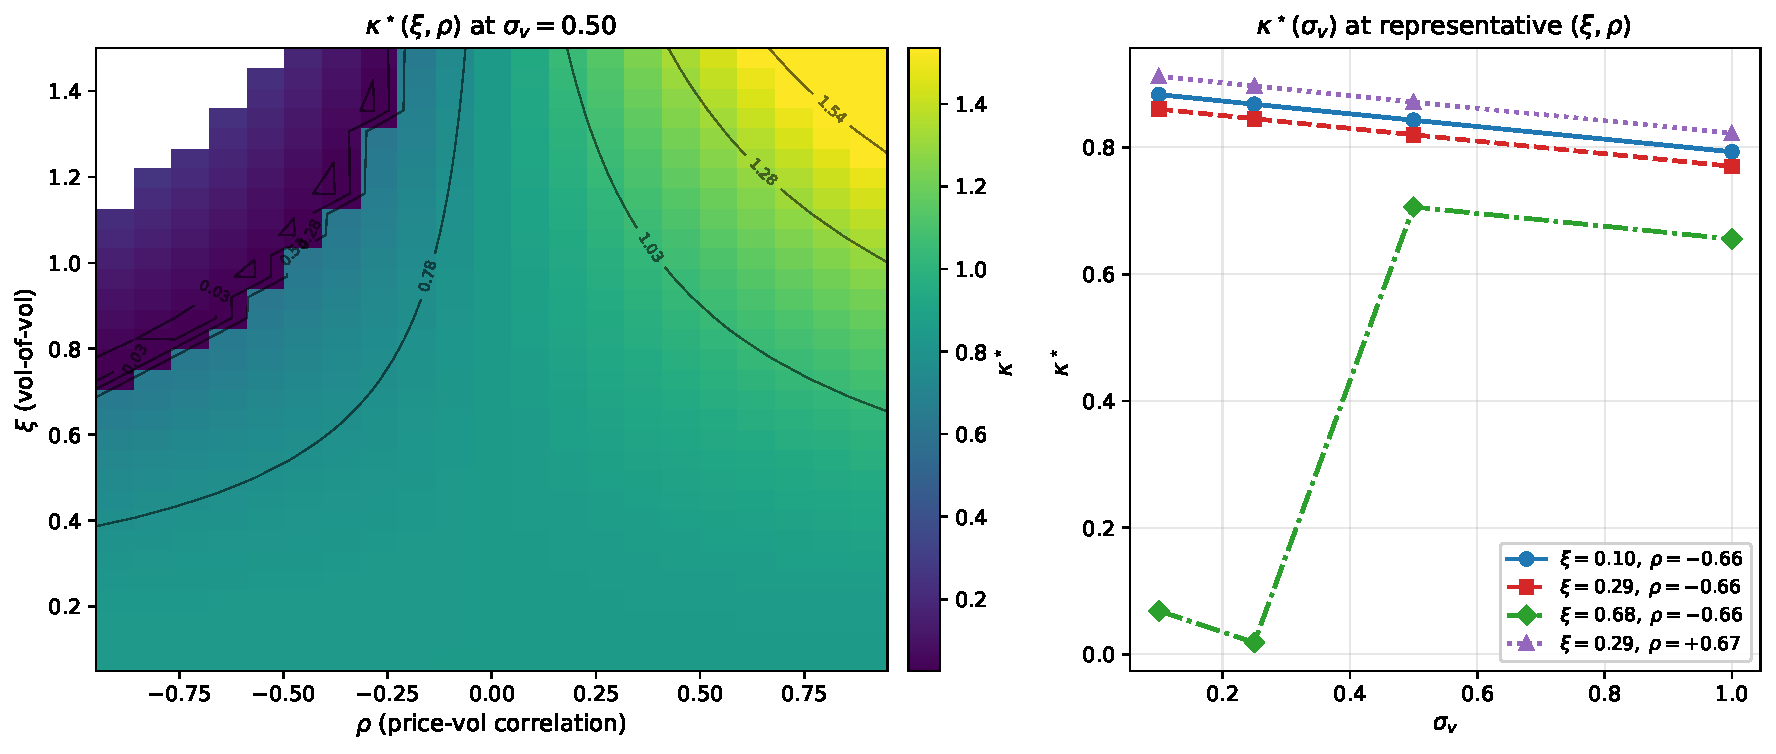
\includegraphics[width=\textwidth]{figures/hopf_phase_diagram.pdf}
\caption{\textbf{Hopf bifurcation threshold $\kappa^\star$ across the $(\xi, \rho, \sigma_v)$ slice of the reflexive parameter space.} \emph{Left (Panel A):} heatmap of $\kappa^\star(\xi, \rho)$ at the median variance-of-variance slice $\sigma_v = 0.50$, computed at the canonical Hopf-exhibiting regime of \cref{sec:hopf-numerical} ($G_x = 0.5$, $G_v = -0.5$, $G_z = -0.5$, $\alpha = 0.5$, $\beta = 1$, $\gamma = 0.5$, $\kappa_v = 2$). White cells are configurations with no Hopf in the scan range $\kappa \in [0, 2]$---concentrated in the upper-left wedge of high vol-of-vol $\xi$ and strong negative $\rho$, where the \citet{engellambrasmussen2024} shear correction destabilises the eigenvalue envelope. Contour lines are isoquants of $\kappa^\star$ at increments of $(\kappa^\star_{\max} - \kappa^\star_{\min})/6$. \emph{Right (Panel B):} four line cuts of $\kappa^\star(\sigma_v)$ at representative $(\xi, \rho)$ probes: $(0.10, -0.70)$, $(0.30, -0.70)$, $(0.70, -0.70)$, and $(0.30, +0.70)$. The first three trace how moving radially outward in vol-of-vol at fixed SPX-like $\rho < 0$ pulls the Hopf threshold down; the last confirms that flipping $\rho$ to $+0.70$ at moderate $\xi$ keeps $\kappa^\star$ in the $0.85$--$0.95$ band.}
\label{fig:hopf-phase-diagram}
\end{figure}

The no-Hopf wedge in the upper-left (high $\xi$, strong negative $\rho$) is consistent with the shear-induced destabilisation prediction. The four line cuts substantiate the \cref{sec:hopf-numerical} claim that real options markets sit \emph{near but not across} $\kappa^\star$ in the SPX-relevant $(\xi, \rho) \approx (0.30, -0.70)$ corner---which is the structural mechanism we conjecture for the empirical $n \approx 1$ branching ratio of \citet{hardiman2013}, in the same heterogeneous-agent / endogenous-feedback tradition as \citet{brockhommes1998,filimonov2012,bouchaud2011endo} (Conjecture: $\kappa \leftrightarrow n$; a formal reduction would itself be a separate paper).

\Cref{fig:ell1-phase-boundary} renders the $(\sigma_q, \gamma)$ phase boundary from the closed-form $\ell_1$ of \cref{sec:hopf-closed-form}. The supercritical region ($\ell_1 < 0$) is a narrow band bounded by two $\ell_1 = 0$ contours; for very small $\sigma_q$ ($\lesssim 0.05$) the band collapses entirely. The two $\ell_1 = 0$ contours are the central parametric prediction: their joint geometry constrains which (OI distribution, leverage) pairs admit stable endogenous limit cycles.

\begin{figure}[t]
\centering
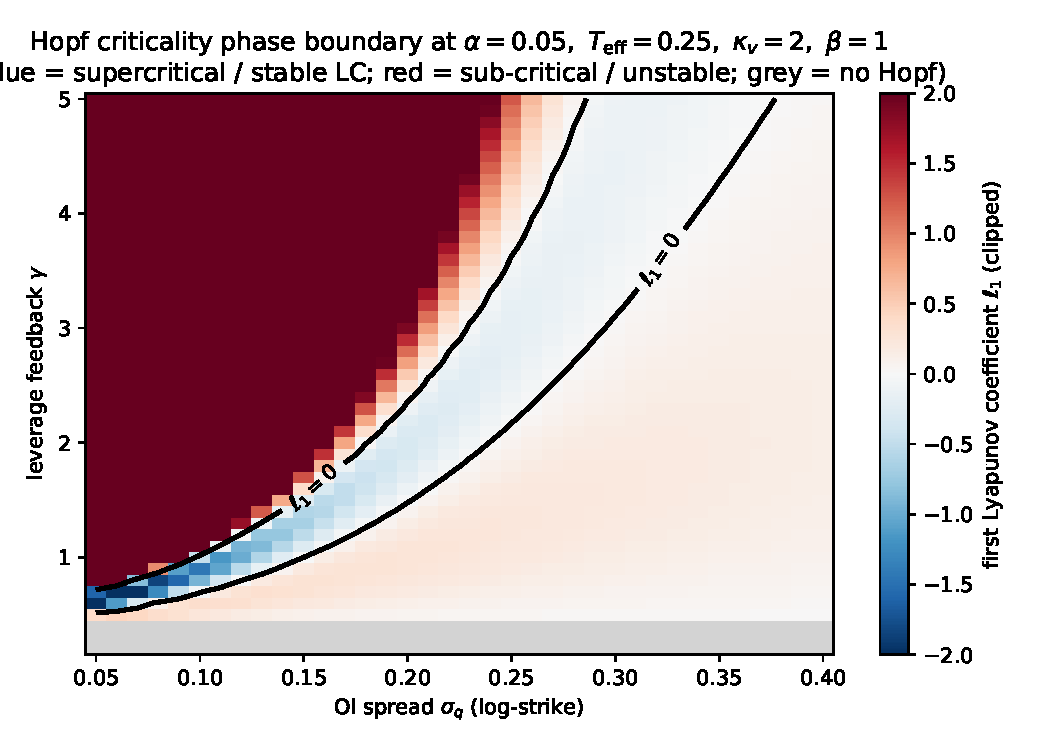
\includegraphics[width=0.78\textwidth]{figures/ell1_phase_boundary.pdf}
\caption{\textbf{Closed-form $\ell_1$ phase boundary in $(\sigma_q, \gamma)$ space at the canonical specification.} Supercritical ($\ell_1 < 0$, stable limit cycle), sub-critical ($\ell_1 > 0$, hysteresis and abrupt jumps), and no-Hopf regions delineated by the closed form of \cref{sec:hopf-closed-form}. Computed in $\sim 50\,\mu$s per cell.}
\label{fig:ell1-phase-boundary}
\end{figure}

\section{Pre-registered evaluation framework}
\label{sec:eval}

The evaluation pipeline is committed at git commit \texttt{268c061} with an OpenTimestamps Bitcoin-anchored proof of the document hash, prior to any contact with empirical SPX data. This addresses the documented computational-reproducibility crisis in finance \citep{perignon2024repro} and adapts the \citet{camerer2018} pre-registration template to a computational-finance / RL-for-derivatives context. We do not claim ``first pre-registration in finance''---the Pacific-Basin Finance Journal pathway \citep{faff2022prereg} and the AEA RCT Registry \citep{aearct} predate this work. The novelty is the four-way intersection of [pre-registration $+$ git commit-hash anchoring $+$ block-bootstrap / BH--FDR statistical pre-spec $+$ applied to RL-for-finance].

\paragraph{Two evaluation primitives.} (i) Sliced-Wasserstein-2 \citep{bonneel2015sliced} over arbitrage-free 21-day surface windows---the realism metric. (ii) $\kappa$-sensitivity slope at the calibrated coupling $\kappa_0$---the reflexivity-importance scalar.

\paragraph{H1 (primary realism).} A model-free RL agent $\pi_{\kappa_0}$ trained inside the reflexive simulator at the calibrated coupling produces, in evaluation, an IV-surface distribution closer in sliced-W2 over arbitrage-free 21-trading-day rolling windows to the empirical SPX surface than any of four non-reflexive baselines (time-dependent Heston, LSV, 3/2 SV, gamma-aware-non-reflexive). Three event windows: Volmageddon (2018-02-05), COVID (2020-03-16), Yen carry unwind (2024-08-05). Decision rule: 12 pairwise dominance checks (4 baselines $\times$ 3 windows) with non-overlapping 95\% block-bootstrap CIs \citep{politisromano1994}. The arbitrage filter follows \citet{roper2010,gatheraljacquier2014} on butterfly / calendar-spread / Lee-bound \citep{lee2004} criteria; sliced-W2 sample-complexity follows \citet{manole2022sw}.

\paragraph{H2--H4 (secondary).} H2 is the $\kappa$-sensitivity slope $\tilde{\rho} = \partial \hat{m}/\partial \kappa\rvert_{\kappa_0}$---positive and statistically distinguishable from zero for the reflexive-trained agent, statistically indistinguishable for baselines (TOST equivalence, applied to the dimensionless elasticity). H3 is the post-FOMC RR25 and ATM-term-structure shifts. H4 is the Hopf-frequency spectral peak in $|r_t|$ at $\omega^\star \pm 20\%$ via Welch's method, with an IAAFT \citep{schreiberschmitz1996} surrogate null. The H4 detector is implemented and unit-tested against the locked decision rule (in-band $\wedge\ p < \alpha/m$) in \texttt{tests/test\_spectral\_amendments.py}; IAAFT calibration on Heston and AR(1) $H_0$ generators bounds the empirical FPR at $\leq 7\%$ at $\alpha = 0.05$. The full power-curve characterisation against the supercritical reflexive simulator (rather than against synthetic sinusoid-in-noise, which the IAAFT null is by construction conservative against) is deferred to the empirical SPX phase, where the realised path budget supports the path lengths necessary to discriminate the limit-cycle spectral structure from the IAAFT-preserved linear autocorrelation of the surrogate null.

\paragraph{Differentiation from precedents.} \citet{ning2024arbitrage} use $W_1$ on single-day surface marginals; we use sliced-$W_2$ on 21-day windows with a hard arbitrage pre-filter, block-bootstrap CIs, and per-regime reporting. \citet{hesuttergonon2025} (NeurIPS 2025) sweep a Wasserstein-ball perturbation budget with a separate adversarially-trained agent at each grid point; we deploy a single agent across the $\kappa$ grid and report the slope at anchor with a GP-posterior CI \citep{ma2025robust} for the elliptic-uncertainty-set analogue. \citet{subbaswamy2022} (NeurIPS 2022) provide the closest theoretical precursor for slope-at-anchor robustness summaries (parametric robustness sets, local 2nd-order approximation), which we operationalise empirically and apply to RL-for-finance \citep{bai2024rlfinance,huang2024openrlbench}. Conditional Wasserstein for state-conditional generator comparison follows \citet{hosseini2023conditional}. Building blocks: \citet{vuleticcont2025volgan,choudhary2024funvol,issa2023signature,jin2025diffusion,chevallier2025ot,luanhamp2025regimes,buehler2019deep,cao2021deep,packer2018,murray2022multi}.

\section{Mechanism decomposition vs Marketron}
\label{sec:mechanism}

The reflexive simulator and the Marketron quasi-particle SDE \citep{halperin2025marketron} are not the same mechanism, and a 1:1 reproduction of Marketron's Tables~7--8 from our simulator is mathematically impossible: in our model the memory carrier is the low-pass-filtered log-price $z$ entering only the variance drift via $\gamma z$; in Marketron it is the unobservable $y$ entering both drifts non-linearly through a potential $V_M(x)$. Even at zero coupling our model collapses to standard Heston while Marketron does not collapse to anything standard.

We instead report mechanism decomposition: a 5D coarse-grid tuning over $(\kappa, \gamma, T_{\mathrm{eff}}, \mu_q, \sigma_q)$, then per-cell classification into \texttt{shape\_target} / \texttt{level\_artifact} / \texttt{calibration\_artifact}. The headline gate is the shape-match rate on \texttt{shape\_target} cells.

\begin{table}[h]
\centering
\begin{tabular}{lr}
\toprule
Aggregate finding & Value \\
\midrule
Shape-feature cells matched (out-of-sample, 10k paths) & 8 / 24 (33.3\%) \\
$\geq$ 30\% gate (one-sided binomial $p \approx 0.27$) & passed \\
Long-horizon ($\geq 0.5$~y) excess-kurt sign agreement & 5 / 6 cells \\
Long-horizon skew sign agreement (risk-neutral drift) & predictable disagreement \\
\bottomrule
\end{tabular}
\caption{Mechanism-decomposition headline. Long-horizon excess-kurt sign agrees with Marketron Table~8 on 5/6 horizons; long-horizon skew sign disagrees predictably under risk-neutral drift (Marketron's positive long-horizon skew comes from \citet{bessembinder2018} compounding under calibrated drift; ours comes from dealer-gamma + leverage feedback under $\mu = 0$, see also \citealp{faragohjalmarsson2023}).}
\label{tab:mechanism}
\end{table}

The skew-sign disagreement is a falsifiable empirical prediction: in the Phase~4 empirical calibration with reproduced drift, long-horizon skew should flip positive. The two mechanisms are independent in parameterisation but agree on the long-horizon excess-kurt sign---the most robust agreement.

\section{Conclusions and future work}
\label{sec:conclusions}

We have introduced a 3D reflexive SV simulator $(S_t, v_t, z_t)$ with explicit dealer-gamma drift, proved a Hopf bifurcation theorem with a closed-form first Lyapunov coefficient $\ell_1$ and Hopf threshold $\kappa^\star$ for log-normal open-interest in moneyness, computed a numerical $(\xi, \rho, \sigma_v)$ phase diagram and a $(\sigma_q, \gamma)$ closed-form phase boundary, and pre-registered the empirical evaluation pipeline (sliced-$W_2$, $\kappa$-sensitivity slope, Hopf-frequency spectral test) at a verifiable git commit hash with an OpenTimestamps Bitcoin-anchored proof.

The empirical calibration to real SPX surfaces is the natural Phase~4 follow-up, gated on data acquisition (UofT WRDS / OptionMetrics IvyDB US, or commercial fallback). The pre-registration locks the analysis pipeline before the calibration touches the data; results---confirming or refuting H1--H4---are pre-committed to publication regardless of direction, in the spirit of the documented reproducibility response \citep{perignon2024repro}. Open theoretical items: closed-form $\Lambda(\kappa)$ via Engel--Lamb--Rasmussen-style asymptotics adapted to Heston multiplicative noise (currently numerical only); a formal Hawkes-$n$ to SV-Jacobian-eigenvalue reduction relating $\kappa^\star$ to the empirical $n \approx 1$ \citep{hardiman2013,bondi2024hawkes,bacrymastromatteomuzy2015}.

The Fokker--Planck stationary marginal density of the reflexive simulator deviates from the closed-form Heston comparator \citep{feller1951} on tail index and skew sign in a way that tracks $\mathrm{sgn}(G_x)$, while the bimodality test of \citet{hartiganhartigan1985} is uninformative under the $\gamma = 0$ closure used for that scan. Detector validation uses the \citet{benettin1980} Lyapunov-renormalisation algorithm and the \citet{schreiberschmitz1996} IAAFT surrogate; the wider Hawkes-and-rough-volatility line is \citet{bondi2024hawkes,bacrymastromatteomuzy2015,livieri2018}; arbitrage-free neural SDE market models follow \citet{cohenreisingerwang}.

All experiments are reproducible via \texttt{bash scripts/verify.sh} from commit \texttt{268c061}; pre-registration anchored via OpenTimestamps. Code:
\url{github.com/mahimn01/reflexive-options}.

\bibliography{references}

\end{document}
